\begin{pastexam}[label={px:ncku-113-prog-09}]{成大資訊聯招 113 學年度 第 9 題}
（單選）

\textbf{[5\%]} Given the following B$^+$-tree of order 4 (2-3-4 tree). The capacity of a data node
is 3 and a data node has at least two elements.
\begin{center}
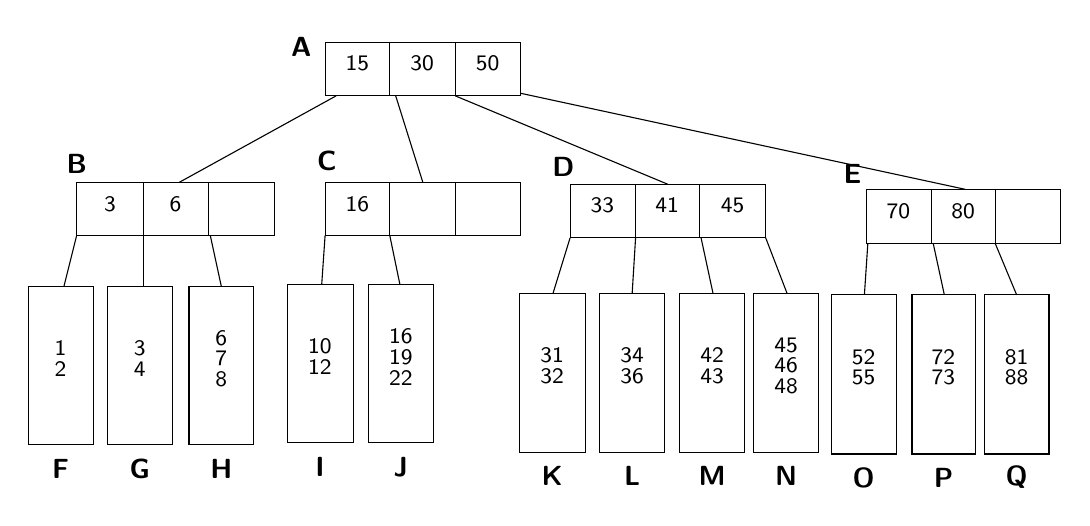
\begin{tikzpicture}[x=0.0108cm,y=-0.0108cm,font=\sffamily\footnotesize,nm/.style={font=\sffamily\bfseries}]
\draw (372,25) rectangle (448,88);
\node at (410,50) {15};
\draw (448,25) rectangle (525,88);
\node at (486,50) {30};
\draw (525,25) rectangle (602,88);
\node at (563,50) {50};
\node[nm] at (344,30) {A};
\draw (80,190) rectangle (158,252);
\node at (119,215) {3};
\draw (158,190) rectangle (235,252);
\node at (196,215) {6};
\draw (235,190) rectangle (312,252);
\node[nm] at (80,168) {B};
\draw (372,190) rectangle (448,252);
\node at (410,215) {16};
\draw (448,190) rectangle (525,252);
\draw (525,190) rectangle (602,252);
\node[nm] at (374,165) {C};
\draw (660,192) rectangle (737,255);
\node at (698,217) {33};
\draw (737,192) rectangle (812,255);
\node at (774,217) {41};
\draw (812,192) rectangle (890,255);
\node at (851,217) {45};
\node[nm] at (652,172) {D};
\draw (1008,198) rectangle (1085,262);
\node at (1046,224) {70};
\draw (1085,198) rectangle (1160,262);
\node at (1122,224) {80};
\draw (1160,198) rectangle (1237,262);
\node[nm] at (992,180) {E};
\draw (23,312) rectangle (100,498);
\node[align=center] at (61,397) {1\\[-2pt]2};
\node[nm] at (61,526) {F};
\draw (116,312) rectangle (193,498);
\node[align=center] at (154,397) {3\\[-2pt]4};
\node[nm] at (154,526) {G};
\draw (212,312) rectangle (288,498);
\node[align=center] at (250,397) {6\\[-2pt]7\\[-2pt]8};
\node[nm] at (250,526) {H};
\draw (328,310) rectangle (405,496);
\node[align=center] at (366,395) {10\\[-2pt]12};
\node[nm] at (366,524) {I};
\draw (423,310) rectangle (499,496);
\node[align=center] at (461,395) {16\\[-2pt]19\\[-2pt]22};
\node[nm] at (461,524) {J};
\draw (601,320) rectangle (678,507);
\node[align=center] at (639,405) {31\\[-2pt]32};
\node[nm] at (639,535) {K};
\draw (695,320) rectangle (771,507);
\node[align=center] at (733,405) {34\\[-2pt]36};
\node[nm] at (733,535) {L};
\draw (789,320) rectangle (865,507);
\node[align=center] at (827,405) {42\\[-2pt]43};
\node[nm] at (827,535) {M};
\draw (876,320) rectangle (952,507);
\node[align=center] at (914,405) {45\\[-2pt]46\\[-2pt]48};
\node[nm] at (914,535) {N};
\draw (967,322) rectangle (1044,509);
\node[align=center] at (1005,407) {52\\[-2pt]55};
\node[nm] at (1005,537) {O};
\draw (1062,322) rectangle (1137,509);
\node[align=center] at (1099,407) {72\\[-2pt]73};
\node[nm] at (1099,537) {P};
\draw (1147,322) rectangle (1223,509);
\node[align=center] at (1185,407) {81\\[-2pt]88};
\node[nm] at (1185,537) {Q};
\draw (385,88)--(200,190);
\draw (455,88)--(487,190);
\draw (525,88)--(775,192);
\draw (602,85)--(1125,198);
\draw (80,252)--(65,312);
\draw (158,252)--(158,312);
\draw (237,252)--(250,312);
\draw (372,252)--(368,310);
\draw (448,252)--(460,310);
\draw (660,255)--(640,320);
\draw (737,255)--(733,320);
\draw (814,255)--(828,320);
\draw (890,255)--(915,320);
\draw (1010,262)--(1006,322);
\draw (1087,262)--(1100,322);
\draw (1160,262)--(1185,322);
\end{tikzpicture}
\end{center}

Which of the following statement is true?
\begin{enumerate}[label=(\Alph*)]
\item After inserting the element whose key is 49 into the B$^+$-tree, 45 becomes in the root.
\item After deleting 72 from the B$^+$-tree, the number of keys in node E is 2.
\item After inserting the element whose key is 28 into the B$^+$-tree, the key in node C is 16.
\item After deleting 45 from the B$^+$-tree, the keys in node D are 33, 41, and 45.
\item None of the above
\end{enumerate}
\end{pastexam}

\begin{pastsoln}
答案是 (D)。

\textbf{約定}（資結書第~11.3~節）。 內部節點（A--E）是 $4$ 階：最多 $3$ 個鍵、$4$ 個子節點，非根的
內部節點至少 $\lceil 4/2 \rceil = 2$ 個子節點（$1$ 個鍵）。 葉子（資料節點 F--Q）放 $2$ 到 $3$ 個鍵。
分隔鍵等於右邊子樹的最小鍵，搜尋 $k$ 時遇到 $k \ge$ 分隔鍵就往右。 葉子溢位時分成兩半，右半的第一
個鍵\textbf{複製}上去；內部節點溢位（$4$ 個鍵 $k_1 < k_2 < k_3 < k_4$）時，$k_1$ 留下、$k_2$
\textbf{移}上去、$k_3, k_4$ 到新節點（資結書第~11.2.4~節，$p = \lceil m/2 \rceil = 2$）。 刪除只從葉子
拿掉鍵，葉子不足 $2$ 個才向兄弟借或合併；內部節點裡的分隔鍵即使在葉子裡已經被刪掉也可以留著。

\textbf{(A) 插入 49}：$30 \le 49 < 50$，走到 D；$49 \ge 45$，走到 N $= \{45, 46, 48\}$。 加入後
$\{45, 46, 48, 49\}$ 溢位，分成 $\{45, 46\}$ 和 $\{48, 49\}$，$48$ 複製到 D。 D 變成
$\{33, 41, 45, 48\}$，溢位：$33$ 留下，$41$ 上移，$\{45, 48\}$ 成為新節點。 A 變成 $\{15, 30, 41, 50\}$，
又溢位：$15$ 留下，$30$ 上移成為新的根，$\{41, 50\}$ 成為新節點。 新的根只有 $30$，$45$ 不在根裡，
(A) 錯。 （如果內部節點分裂時改成讓左邊留兩個、上移第 $3$ 個鍵，D 會上移 $45$、A 也會上移 $45$，
(A) 就變成對的；但那樣 (A)、(D) 都對，和單選不合，所以題目用的是上移第 $2$ 個鍵的約定。）

\textbf{(B) 刪除 72}：P $= \{72, 73\}$ 變成 $\{73\}$，不足 $2$ 個。 兩個兄弟 O $= \{52, 55\}$、
Q $= \{81, 88\}$ 都只有 $2$ 個，借不出來，只能合併：和 O 合併成 $\{52, 55, 73\}$，E 拿掉分隔鍵
$70$ 剩 $\{80\}$；或和 Q 合併成 $\{73, 81, 88\}$，E 拿掉 $80$ 剩 $\{70\}$。 E 還有 $2$ 個子節點，合法，
不必再往上調整。 兩種做法 E 都只剩 $1$ 個鍵，(B) 錯。

\textbf{(C) 插入 28}：$15 \le 28 < 30$，走到 C；$28 \ge 16$，走到 J $= \{16, 19, 22\}$。 加入後
$\{16, 19, 22, 28\}$ 溢位，分成 $\{16, 19\}$ 和 $\{22, 28\}$，$22$ 複製到 C，C 變成 $\{16, 22\}$。 C 有
$16$ 和 $22$ 兩個鍵，不是只有 $16$，(C) 錯。

\textbf{(D) 刪除 45}：$45 \ge 45$，走到 N $= \{45, 46, 48\}$，拿掉 $45$ 剩 $\{46, 48\}$，仍有 $2$ 個，
不必借也不必合併，內部節點都不用動。 D 裡的分隔鍵 $45$ 仍然正確地分開 M（鍵都 $< 45$）和 N（鍵都
$\ge 45$），留著即可。 所以 D 仍是 $33, 41, 45$，(D) 對。 （有些寫法會順手把分隔鍵改成 N 新的最小鍵
$46$，那是選擇性的；照 B$^+$ 樹的一般做法，刪除不會改到內部節點。）

(E) 錯，因為 (D) 對。
\end{pastsoln}
